\graphicspath{{Chapter3/Figs/}}
\nobibliography*

\chapter[Analysis of Area Oscillations]{Analysis of Area Oscillations\footnote{This chapter is based on \bibentry{Dorotovic2014}. Reproduced with permission from Astronomy \& Astrophysics, © ESO}}
\label{chapter3}

   \vspace*{\fill}\par
   \pagebreak

\section{Introduction}

	Chapter 1 details the theory and thus the mechanism to observe MHD sausage modes within magnetic flux tubes. 
	The basic MHD theory has been developed since the early 1970's, as such, sunspots have been intensively studied for oscillations. 
	The commonly studied oscillatory periods in sunspots are three and five minutes.
	These oscillations are seen in intensity, line-of-sight (LOS) velocity, and LOS magnetic field.
	Moving away from LOS oscillations required more understanding of MHD wave theory in cylindrical flux tubes. 

	The MHD sausage mode are of interest here, because the sausage mode is a compressible, symmetric perturbation around the axis of a flux tube that causes density perturbations that can be identified in intensity images \citep{PMHDW}.
	Furthermore, because the wave will either compress or expand the flux tube, the magnetic field will also show signs of oscillations.
	This mode may come in two forms in terms of phase speed classification: the slow mode (often also called the longitudinal mode), which generally has a phase speed close to the characteristic tube speed and, the fast mode which has a phase speed close to the external sound speed.
	One of the main differences between the two modes is the phase relationship between appropriate MHD quantities which allows them to be differentiated.
	In this case, the fast sausage mode has an out of phase relationship between the cross-sectional area and total intensity, while the slow sausage mode has an in phase relationship.
	The technique that was applied to obtain these phase relationships are covered by, \cite{PMHDW}, \cite{Moreels2013}, and \cite{Moreels2013b}.

	Sausage modes have been observed in magnetic pores before.
	\citet{doretala2008} observed a magnetic pore for 11 hours and reported periodicities in the range of 20-70 minutes.
	These oscillations were consequently interpreted as linear low-frequency slow sausage waves.
	\citet{morton2011} used the Rapid Oscillations in the Solar Atmosphere (ROSA) instrument to also identify linear sausage oscillations in a magnetic pore.
	However, determining whether the oscillations were slow or fast proved to be difficult.

	The source and driving mechanism(s) of these MHD sausage modes have been very difficult to identify.
	Numerical simulations of a flux tube rooted in the photosphere, which is buffeted by a wide range of coherent sub-photospheric drivers, is one method for identifying the potential source of MHD sausage waves.
	These drivers can either be horizontal or vertical, single, or paired or else a power spectrum, with varying phase differences \citep[see e.g.][]{malins,khomenko,fedun2,fedun1,Vigeesh2012}.
	To understand these MHD sausage oscillations, it is necessary to firstly see if it is possible to identify the signature within solar magnetic waveguides situated in the lower solar atmosphere.
	
\section{Data collection and method of analysis}

	\begin{sidewaysfigure}
        
		\centering
		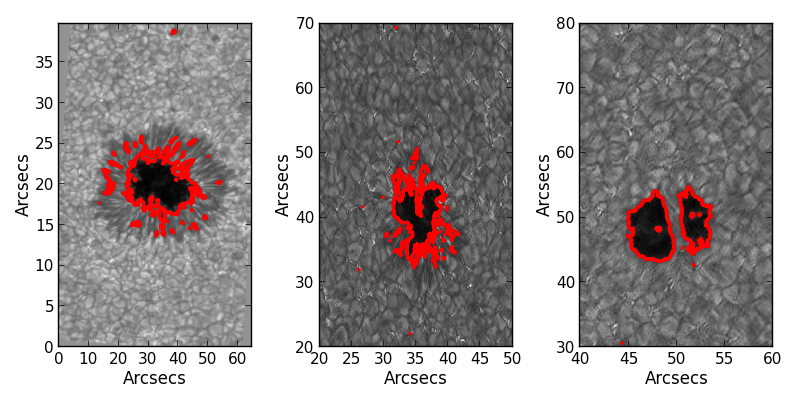
\includegraphics[width=\textwidth]{overview.png}
		\caption{
		An overview of the magnetic waveguides used for this analysis.
		\textit{(left)} The 1999 sunspot observed with the SVST with an average umbral area of 19,650 pixels (50 M km$^{2}$).
		\textit{(middle)} The 2005 sunspot observed with the DOT with an average umbral area of 12,943 pixels (32 M km$^{2}$).
		\textit{(right)} The 2008 pore observed with the DOT with an average area of 10971 pixels (27 M km $^{2}$), the light bridge that separates the pore can be seen.
		Furthermore, these structures were seen near the disk centre, so there is little to no LOS effect.
		The red line shows the thresholding technique applied to each waveguide at the start of each data series.}
		\label{images}
	\end{sidewaysfigure}

	Three time series of images with high angular resolution have been chosen here in order to demonstrate the identification of MHD sausage waves.
	The images were taken in the G-band ($430.5$ nm), which samples the low photosphere.
	This line forms deep in the photosphere and has a line intensity defined as $\rho{^2} \times$ line-of-sight column depth.
	
	The images were acquired using:

	\begin{enumerate}
		\item 
			The Swedish Vacuum Solar Telescope (SVST) situated on La Palma in the Canary Islands.
			\citet{scharmer} provides a detailed description of the features of the SVST.
			The images were taken on 7 July 1999.
			The sunspot is in Active Region (AR) NOAA 8620.
			The observing duration is 133 minutes with a cadence time of 25 seconds.
			The field of view (FOV) covers an area of $33,600$ km by $54,600$ km ($1$ pixel $\approx$ $60$ km). \citet{bonet} gives a detailed analysis of this sunspot.
			A context image is the left-handed image of Figure \ref{images}.
		\item 
			The Dutch Open Telescope (DOT) is also situated on La Palma in the Canary Islands.
			Two series of imaging data sequences were taken using this telescope.
			A detailed guide of the features of the DOT is  provided by \citet{rutten}.
			The first series of data were taken on 13 July 2005, and the sunspot is in the AR NOAA 10789.
			The region slowly decayed, and this sunspot led a small group of other magnetic structures.
			The observing length is 165 minutes and has a cadence time of $30$ seconds.
			The second set of data taken on 15 October 2008 is of a large magnetic pore with a light bridge which is about 15 pixels (750 km) wide in AR NOAA 11005.
			The duration of the observing run is 66 minutes and has a cadence time of $20$ seconds.
			Both DOT image sequences cover an area of $50,000$ km by $45,000$ km, where the maximum spatial resolution is 0.2" ($\approx$ $140$ km).
			Typical context images are the middle and right-handed panels of Figure \ref{images}.
   \end{enumerate}
   
	To obtain information relating to the cross-sectional area of these waveguides, a strict and consistent definition of the cross-sectional area is required.
	The definition is that each pixel with a value of less than $3\sigma$ of the median background intensity is counted as part of the waveguide.
	The background is defined as an area of the image where there are no magnetic features.
	This may appear to be an arbitrary definition; however, a histogram of the background intensity reveals a Gaussian distribution, and when adding the area around and including the waveguide, there is significant peak on the lower end of the Gaussian distribution curve around 3$\sigma$ or higher.
	Thus, we have a $99\%$ confidence that the area is of the structure and not of the background.
	
	Figure \ref{images} shows each waveguide at the start of the time series, where the red contour line represents the regions of cross-sectional area found.
	The definition is accurate, but, it does include some non-waveguide pixels.
	In order to reduce this factor, a bounding box is taken as close to the magnetic waveguides as possible without covering up umbral pixels.
	The total intensity was determined by summing over the intensity of each pixel found in the waveguide.
	These waveguides are not static structures as they slowly changed in size during the observing period.
	This background trend has to be removed for it not to mask any weak oscillatory signatures.
	The detrending was accomplished by a non-linear regression fit and the consistency of the results was compared to subtracting the residue from an empirical mode decomposition (EMD) analysis (explained below).
	The residue is the data that remains after the EMD procedure has extracted as many signals as possible and it provides a very good approximation of the background trend.
 
	The resulting reduced data series were then analysed with a wavelet tool in order to extract any periods of oscillation present within these signals.
	The algorithm used is an adapted version of the IDL wavelet routine developed by \citet{torrence}.
	The standard Morlet wavelet, which is a plane sine wave with an amplitude modulated by a Gaussian function, was chosen for its suitable frequency resolution.
	The white cross-hatched area marks the cone of influence (COI), where edge effects of the wavelet structure affect the wavelet transform, and anything inside the COI is discarded.
	The white dashed line contour shows the confidence level of 95\%.
	The wavelet method is very susceptible to noise at short periods and at times may not identify the true power of short periods.
	
	Beyond this, the data representing the size and intensity has also been analysed using EMD, which decomposes the time series into a finite number of intrinsic mode functions (IMFs).
	IMFs are essentially narrowband-filtered time series, with each IMF containing one or two periods that exist in the original signal.
	The EMD technique was first proposed by \citet{huang} and offers some benefits over more traditional methods of analysis, such as wavelets or Fourier transforms.
	However, one drawback is that it is very prone to error with regards to long periods.
	The problems associated with both the wavelet and EMD process means that the two complement each other.
	Furthermore, periods that appear in the wavelet \textit{just} below the confidence level, but appear strongly in the EMD process, is a good indication that a period is not spurious.
	Generally, the next step after EMD analysis is to construct a Hilbert power spectrum that has a better time and spatial resolution than either wavelet or FFT routines.
	However, this has not been carried out owing to a lack of a robust code base at this time.
	At this stage, we rely on wavelet and EMD analyses, as is customary in solar physics.

\section{Results and discussion}

\subsection{LOS, circularity, and evolution of the waveguide}

    \begin{sidewaysfigure}
		\centering
        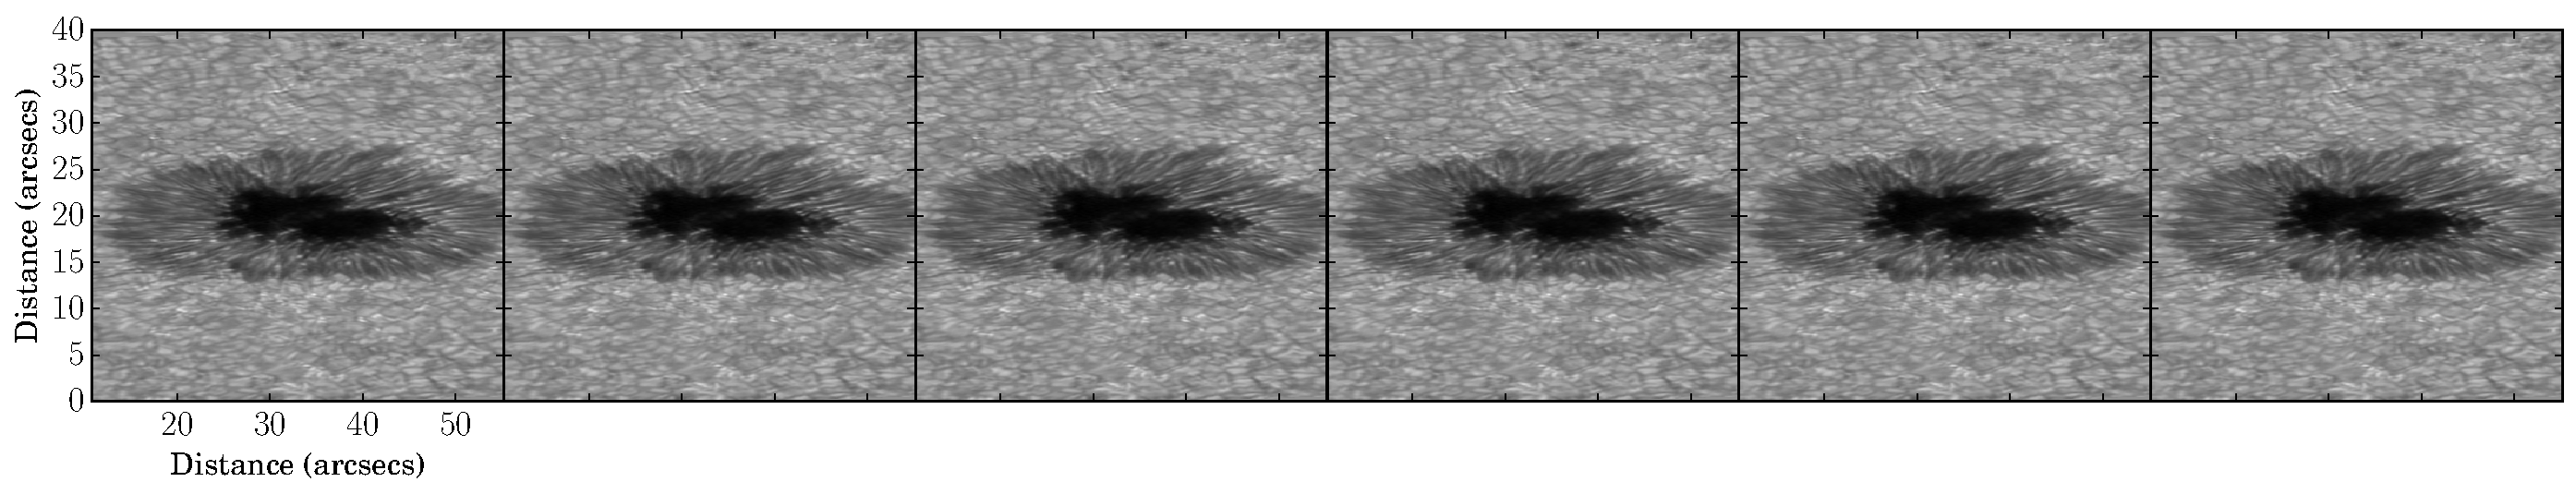
\includegraphics[height=0.19\textheight,width=\textwidth]{1999.pdf}\vspace*{-0.2cm}
        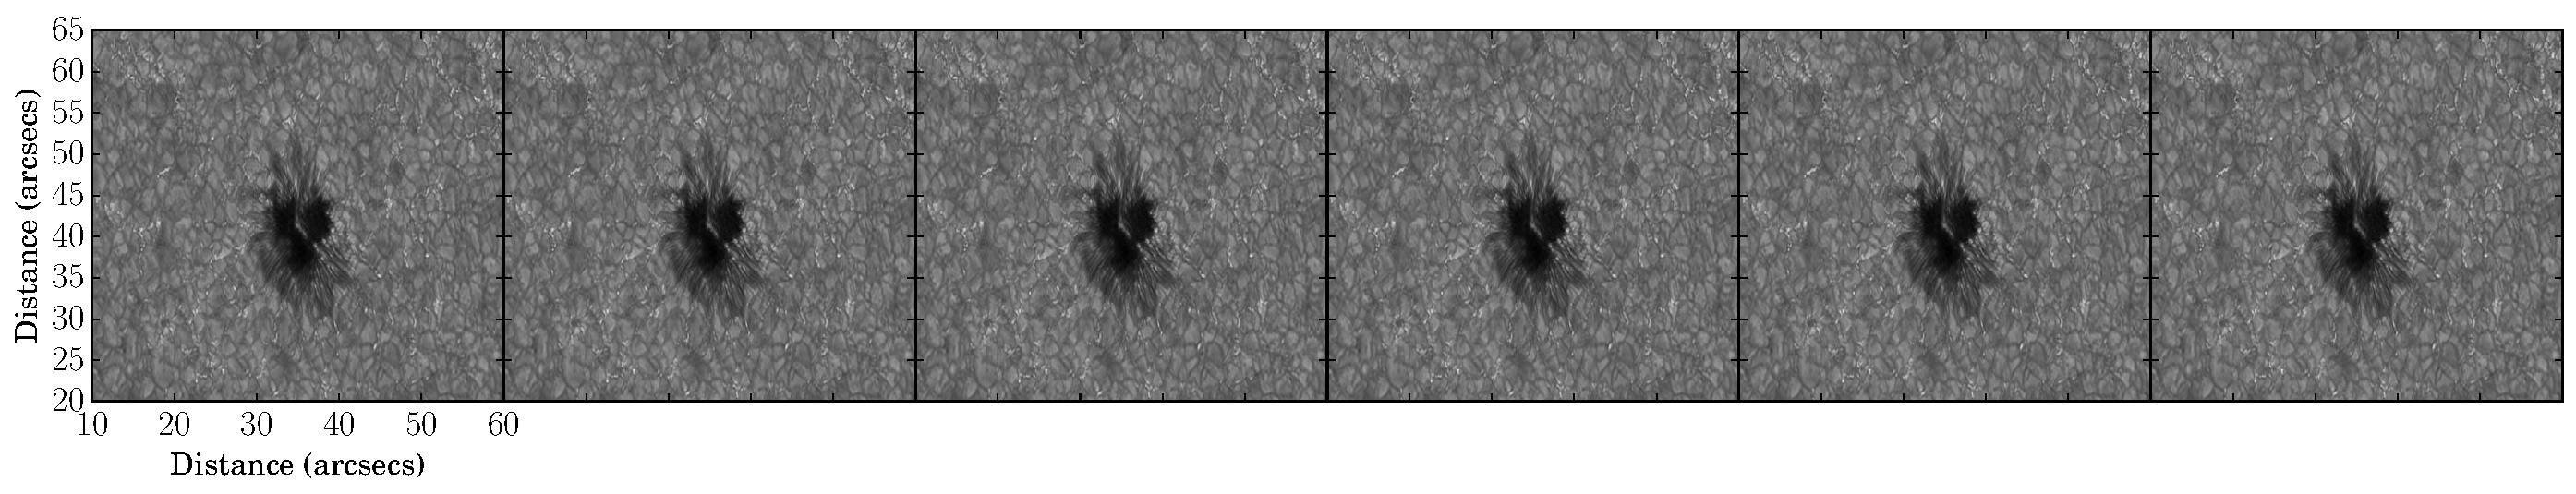
\includegraphics[height=0.19\textheight,width=\textwidth]{2005.pdf}\vspace*{-0.2cm}
        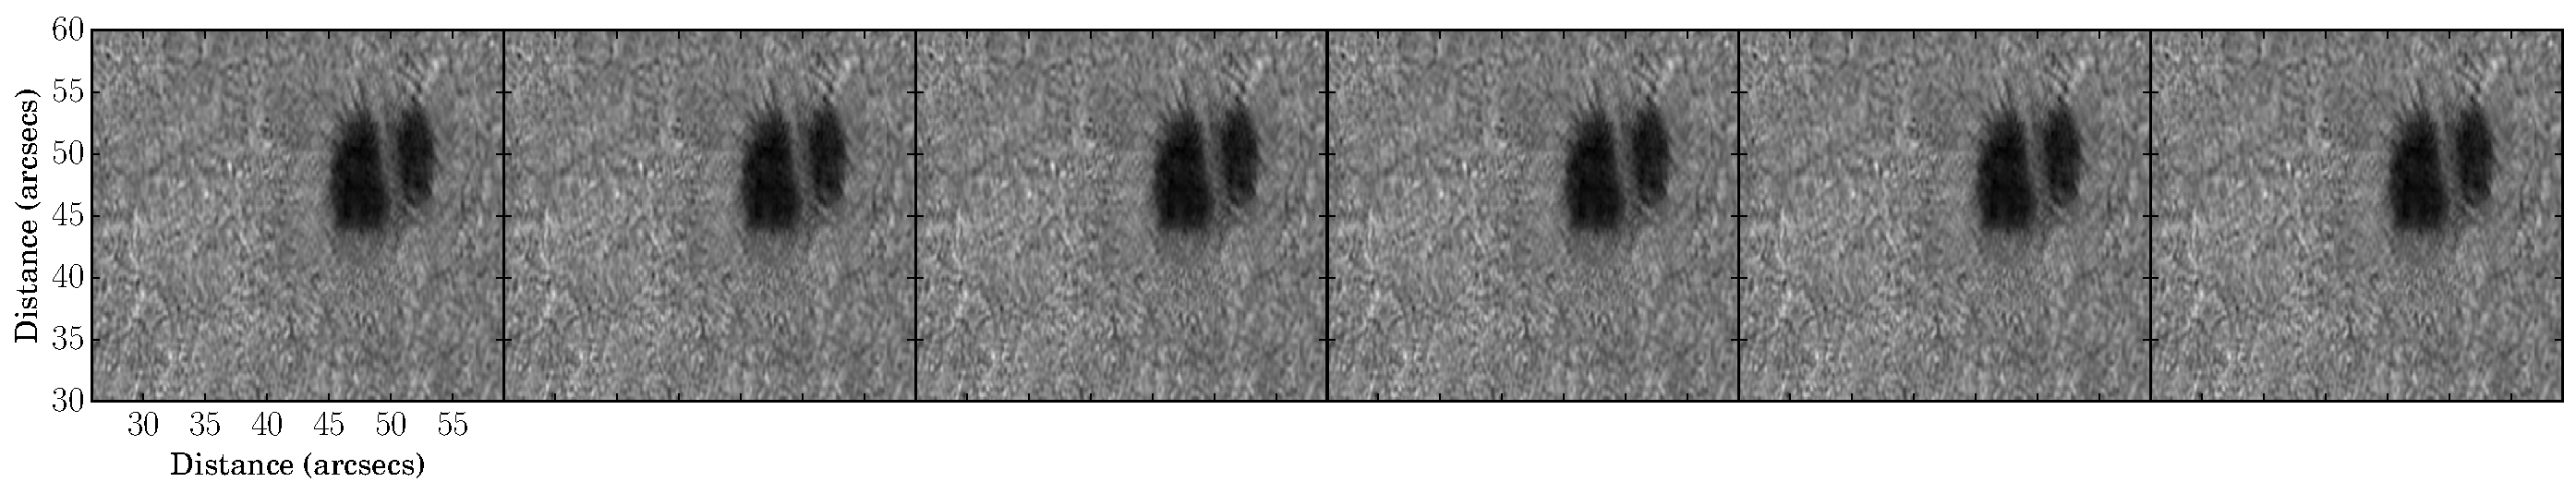
\includegraphics[height=0.19\textheight,width=\textwidth]{2008.pdf}\vspace*{-0.2cm}
        \caption{
            The three waveguides seen through six different parts of their corresponding observation sequence.
            The image sequence has time increasing from left to right.
            The first row is the 1999 sunspot, the middle row the 2005 sunspot, and the last row the 2008 pore.
                }
        \label{data}
    \end{sidewaysfigure}
	
	Several points need to be clarified for the data presented here before the full analysis.
	Firstly, there are LOS issues, \citet{2003A&A...397..765C,2003A&A...409..325C} have investigated how the LOS angle affects various aspects of observing coronal loops in a 2D model.
	Overall they found that for the slow sausage MHD wave, for a range of angles from $\pi/6$ to $\pi/3$, the observed intensity decreases as the LOS angle increases.
	Secondly, the larger angles lengthened the \textit{observed period} of the wave.
	While the objects here are not coronal loops, the LOS angle still matters and should behave similarly.
	The LOS angles in all three cases were less than 30$^\circ$ thereby limiting any relevant effects of LOS.
	
	Sunspots or magnetic pores are not fully circular and can have arbitrary shapes.
	The effects of a non-circular shape have been studied by, for example, \citet{2003A&A...409..287R}, \citet{2009A&A...502..315M}, and \citet{2011A&A...527A..53M}.
	While they do not account for the very complicated and real structure of the sunspots and magnetic pores observed here, they still offer an adequate insight.
	Current theory suggests the shape will have a minor effect on the oscillations unless it has a significant deviation from circularity.
	Likewise, the structure of each waveguide undergoes a minor change during the observation campaign, limiting any effects from large-scale structural change, as can be seen in Figure \ref{data}.

\subsection{MHD theory for phase relations}
	
	Treatment of the MHD equations makes it possible to determine phase relations between various physical quantities for propagating and standing MHD waves.
	This has been summarised briefly by \citet{goedbloed} and also applied by \citet{PMHDW}.
	The latter find that the phase relation for the slow MHD wave with regards to cross-sectional area and density is in phase regardless of whether the wave is propagating or standing.
	More recently, \citet{Moreels2013} have expanded on this idea, taking factors into account such as LOS, which were neglected earlier, but also expanding the theory to cover fast MHD sausage waves.
	The phase relation for the magnetic field to the cross-sectional area is in phase when assuming that the magnetic field is frozen into the plasma.
	
	Supplementary information from other perturbation phase relations, such as the LOS velocity and the LOS magnetic field, allows one to determine whether the observed MHD wave is slow or fast.
	In summary, the slow MHD sausage mode shows in phase behaviour between intensity and area perturbations, while the fast sausage mode shows out of phase behaviour.
	Before progressing, we need to address the opacity effect on MHD wave perturbations.
	This is relevant, since intensity fluctuations can be due to the change of the optical depth along the LOS, which has the same phase difference as the fast MHD sausage wave and as a result is indistinguishable without further information \citep{PMHDW}.
	
	Recently, \citet{Moreels2013b} have analytically determined the phase difference between the cross-sectional area and the total intensity perturbations for both the slow and fast MHD sausage modes.
	Note that any mention of the area means the cross-sectional area from here on in and the intensity means the total intensity.
	They find that, for both the slow body and surface MHD wave, the behaviour is in phase, while for the fast surface wave, the behaviour is out of phase.
	This result means that it is possible to approximately separate slow and fast sausage waves without the use of other observable variables. Their results will be used here to distinguish between slow and fast MHD sausage modes.

\subsection{Sunspot, 7 July 1999 , AR 8620}

   \begin{sidewaysfigure}
	   \centering
       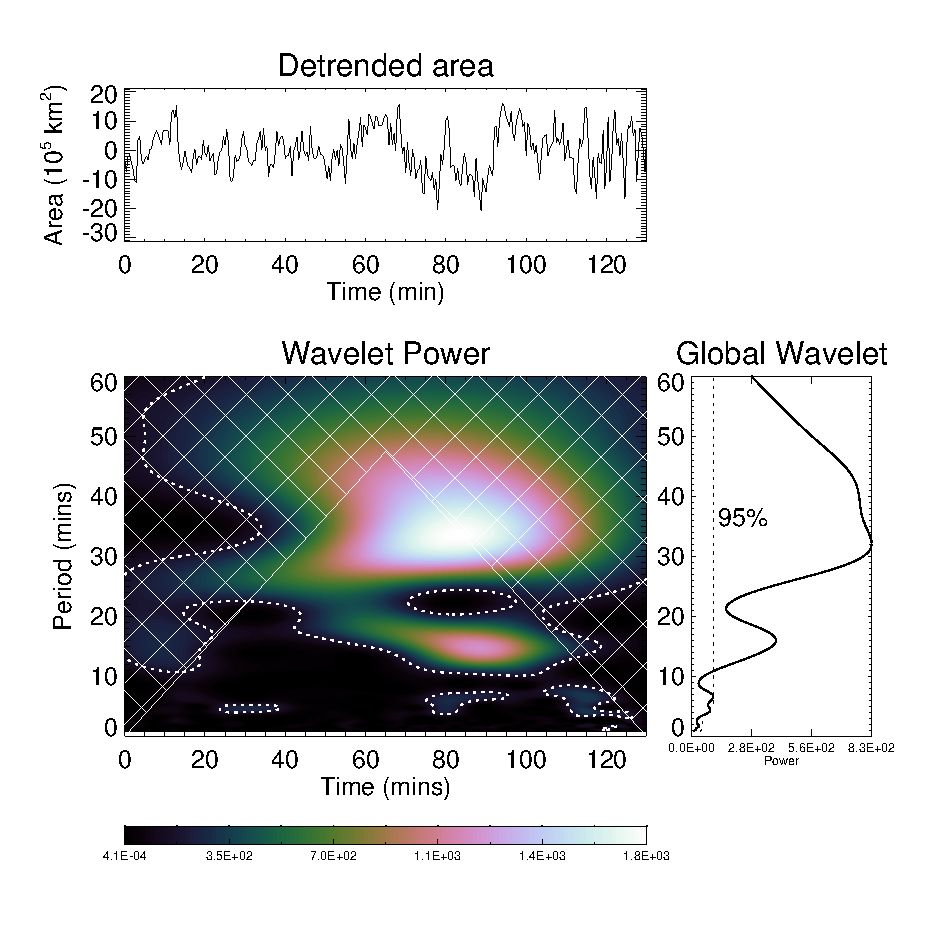
\includegraphics[width=0.49\textwidth]{1999_wl.eps}
       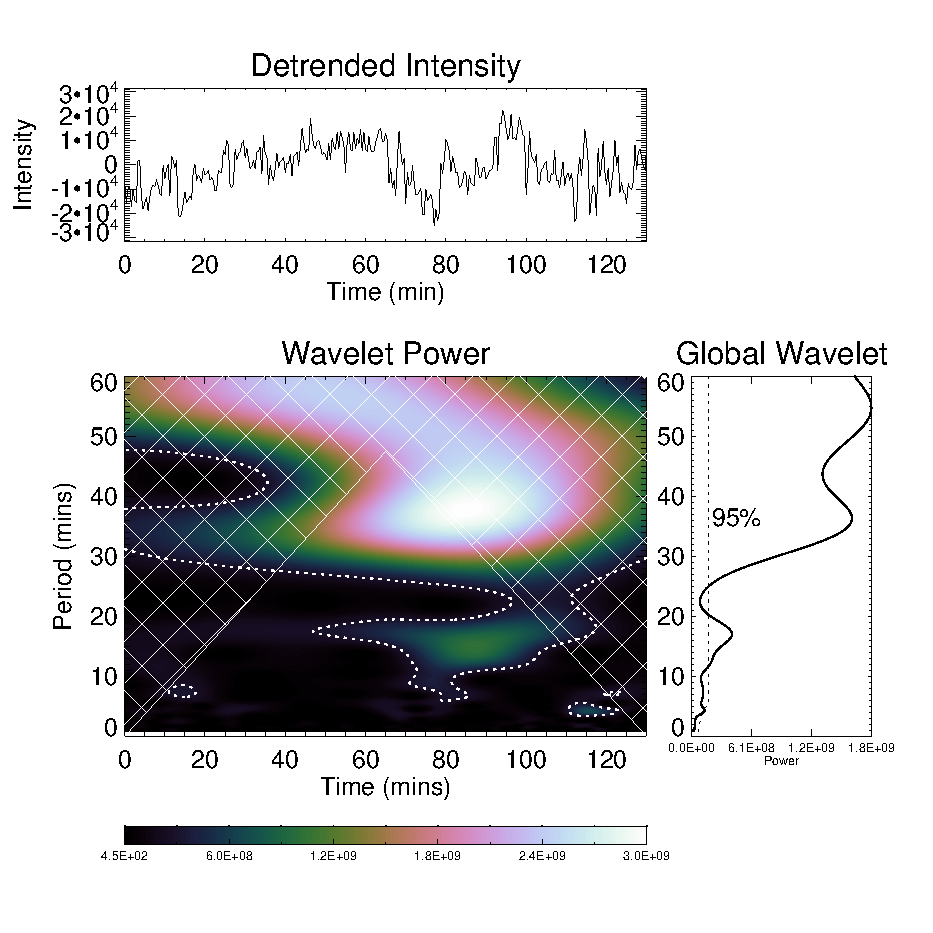
\includegraphics[width=0.49\textwidth]{1999_wl_inten.eps}
	   \caption{
				\textit{(left image)} Evolution of the area of the 1999 sunspot.
				\textit{(right image)} The same as the left image but for the total intensity of the 1999 sunspot.
				\textit{(upper panel)} The signal that is analysed.
				\textit{(lower panel)} The wavelet power spectrum for a white noise background, the cone of influence is marked as a cross-hatched area where edge effects become important and the contour lines show the 95\% confidence level.
				\textit{(lower right panel)} Global (integrated in time) wavelet power spectrum, where the dashed line shows the 95\% confidence limit.   
				}
	   \label{1999sunspot}
   \end{sidewaysfigure}
   	
	Figure \ref{1999sunspot} shows the wavelet analysis of the 1999 sunspot's area and intensity data. There are four confidently identified periods that exist in the area wavelet with 95\% certainty; 4, 7, 16, and 32 minutes.
	The 32-minute period is found over a wide range of the time series, with some of its power inside the COI.
	However, most is outside the COI.
	The 16-minute period is strongly localised at 50 to 120 minutes of the data series, starts at 18 minutes, and slowly increases and stabilises at 14 minutes.
	There is a third and fourth period at four and  seven minutes that just reach the significance level and appear sporadically during the time series.
	
	The intensity wavelet shows three distinct periods of oscillations above the confidence level: 4, 16, and 36.5 minutes.
	The 36.5-minute period has a corresponding area wavelet oscillation at 32 minutes.
	While the 16-minute oscillation corresponds to the 16-minute oscillation found in the area.
	Furthermore, the 16-minute period starts with very concentrated power and does not display the same period change as the area oscillation does.
	Finally, the four-minute period also corresponds to an oscillation found in the area but is also sporadic in its appearance.
	
	It is safe to say that these oscillations are caused by sausage waves.
	The reason is that in linear ideal MHD theory, the sausage wave is the only MHD wave capable of changing the area of the flux tube that is observed on disk \citep[see e.g.][]{2003A&A...397..765C,CLOO}.
	Without the ability to directly compare the phase difference of the area to the intensity, great caution needs to be exercised to determine with confidence whether the perturbations are fast or slow.
	A wavelet phase diagram reveals regions (where the wavelet coherence is high and the period is $\le 20$ minutes) to be either out of phase or in phase, but a clear image of constant phase difference does not appear.
	This might be due to mode conversion occurring in the sunspot, since the G-band samples a region where the plasma-$\beta$ $\approx 1$ in a magnetic structure \citep{gary}.
	When the period is $\ge 20$ minutes, the only area of high coherence is located around 30 minutes and found to be nearly out of phase, which hints that there might be a fast surface sausage wave.
	However, only two full wave periods are outside the COI, which is due to the total length of the data series.
	This behaviour indicates that for short periods, a mixture of fast surface and slow MHD sausage waves are present while for the long period, it is purely a fast surface MHD sausage wave.
		
	
	\begin{sidewaysfigure}
	\centering
	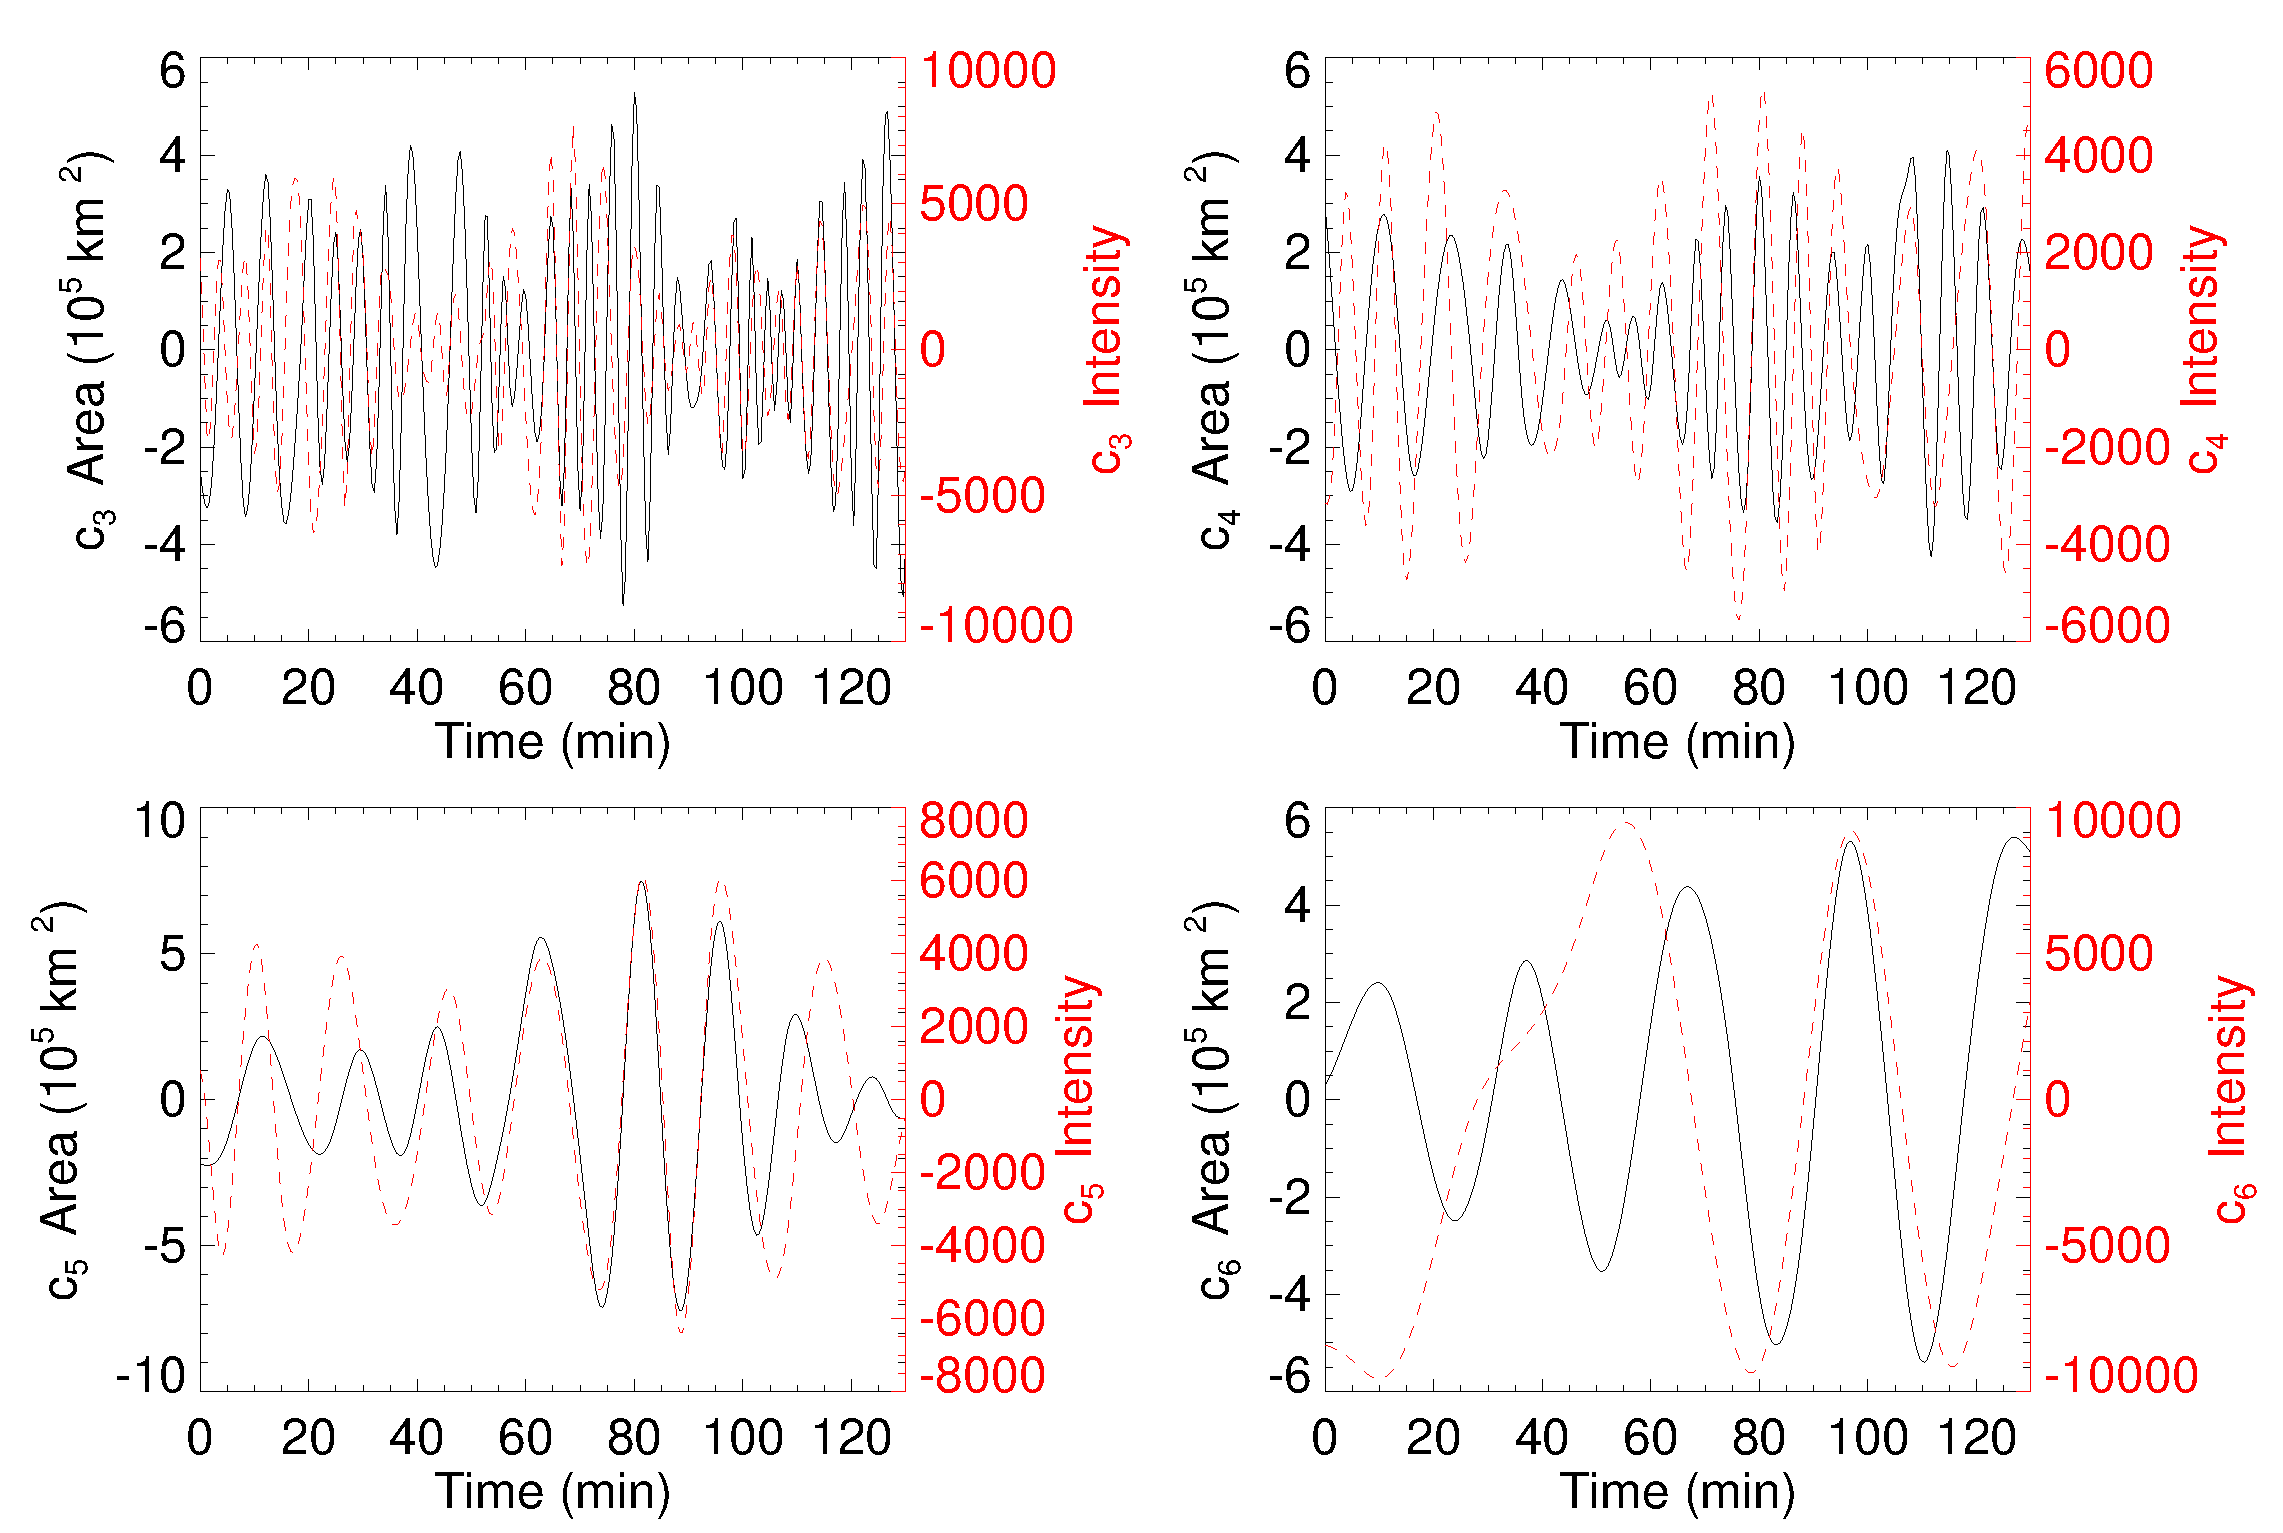
\includegraphics[width=\textwidth]{1999_IMFs.eps}
    \caption{
	      	The IMFs of the evolution of the area (red) and intensity (black) for the 1999 sunspot, over-plotted to aid comparison.
	      	Generally after the $6$th IMF, higher IMFs lack a sufficient number of wave periods, which makes it difficult and less reliable to obtain an accurate period.
   		    }
    \label{1999IMF}
	\end{sidewaysfigure}
		
	Figure \ref{1999IMF} shows the computed IMFs for the 1999 sunspot data set.
	The IMFs show the periods of oscillations identified using the EMD algorithm.
	IMFs which show irrelevant periods, or the residual signal which are ignored.
	In general, the higher order IMFs tend to show longer periods and, as such, contain fewer wave periods, which makes phase identification less reliable.
	Four IMF overlays are shown, and IMFs with similar periods to the wavelet plots have been overlaid in order to aid comparison for each dataset.
	
	Four IMFs directly coincide with the wavelet period that reveal both area and intensity perturbations.
	IMF $c_{3}$ displays the four-minute period where major regions of in phase behaviour can be seen; however, both side shows one or two wave periods of out of phase behaviour.
	IMF $c_{4}$ exhibits a period of seven minutes.
	The picture here is more muddled as an extra period is present in the intensity, namely 11 minutes, making phase identification harder for the seven-minute period.
	Where the IMFs coincide with the same period, namely at the start of the time series, the phase difference is approximately 45 degrees, which the authors have no theoretical explanation for.
	IMF $c_{5}$ displays a 16-minute period, with in phase behaviour.
	Finally, IMF $c_{6}$ contains the 32-minute period.
	This period does not fully match the period seen in the intensity, but also one of the edge effects of the EMD process can be seen in the intensity signal.
	Near the end of the time series, the two IMFs overlap with the same period with an in phase behaviour.
	In summary, the EMD process shows that the major behaviour is in phase, indicating the existence of a slow sausage mode.
	Also the regions of changing phase difference at lower periods indicates the potential existence of a fast surface mode.
	However, the last IMF does not agree with the wavelet phase due to the artefact from the EMD process.
	
	It was possible to approximately separate the penumbra from the umbra and investigate its area for oscillations.
	However, the penumbra is a highly dynamic object and this makes the area estimation reasonably uncertain.
	There seem to be four periods that exist at 95 \% certainty: 5, 9, 15, and 25.
	The three shorter periods (5, 9, and 15 minutes) closely correspond to the 4, 7, and 16-minute oscillations in the umbra; they could be a continuation of these umbral periods that became up-shifted as they enter the less compact structure of the penumbra.
	While the 25-minute period does not directly correspond to an observed area oscillation.
	The wavelet phase analysis shows large regions of out of phase behaviour where the period is either below ten minutes or above 20 minutes.
	This behaviour is a mixed collection of fast surface and slow sausage modes, with regions moving from one phase difference to another after three or more wave periods.

\subsection{Sunspot, 13 July 2005, AR 10789}
   
   \begin{sidewaysfigure}
   \centering
   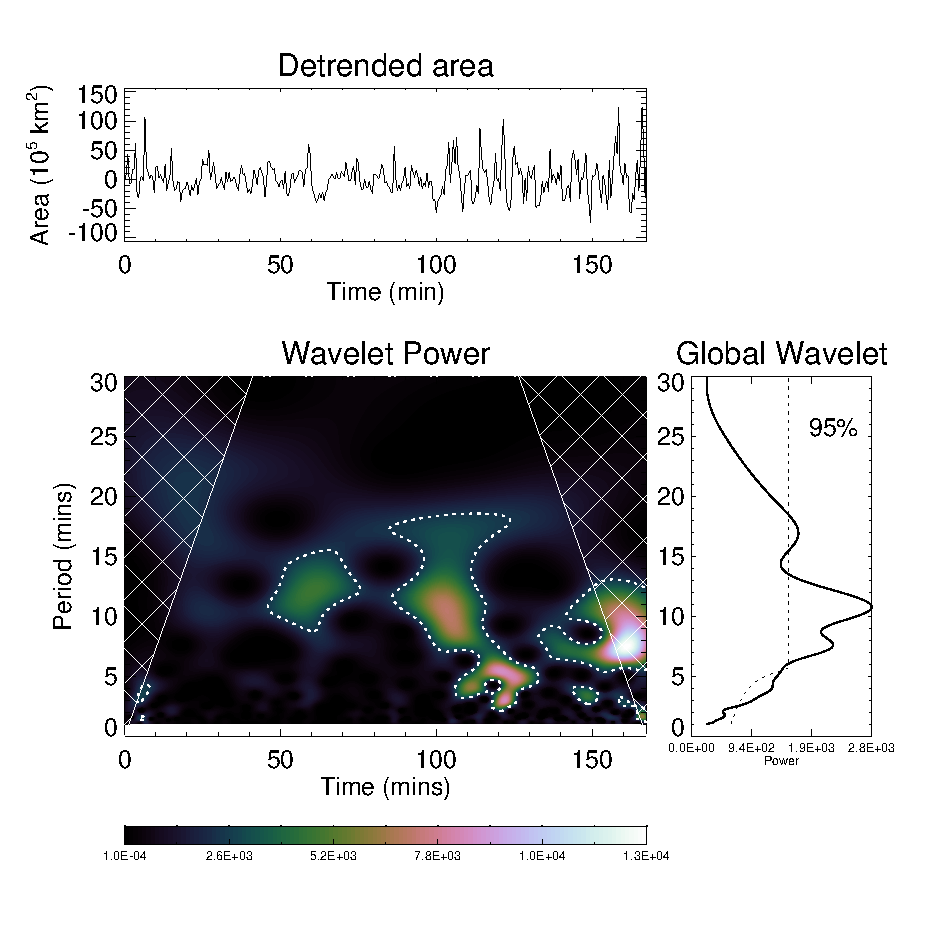
\includegraphics[width=0.49\textwidth]{2005_wl.eps}
   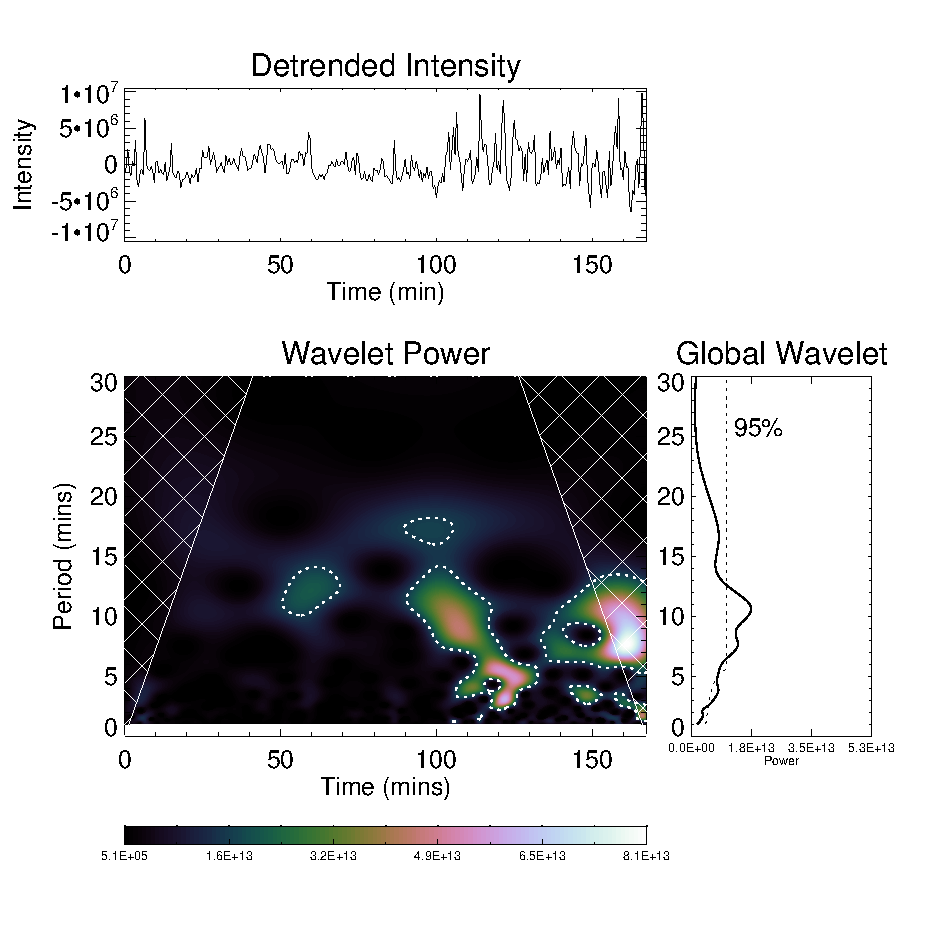
\includegraphics[width=0.49\textwidth]{2005_wl_inten.eps}
      \caption{
      			Same as Figure \ref{1999sunspot} but for the sunspot in AR 10789 observed in 2005.
      		  }
      \label{2005sunspot}
   \end{sidewaysfigure}

   \begin{sidewaysfigure}
   \centering
   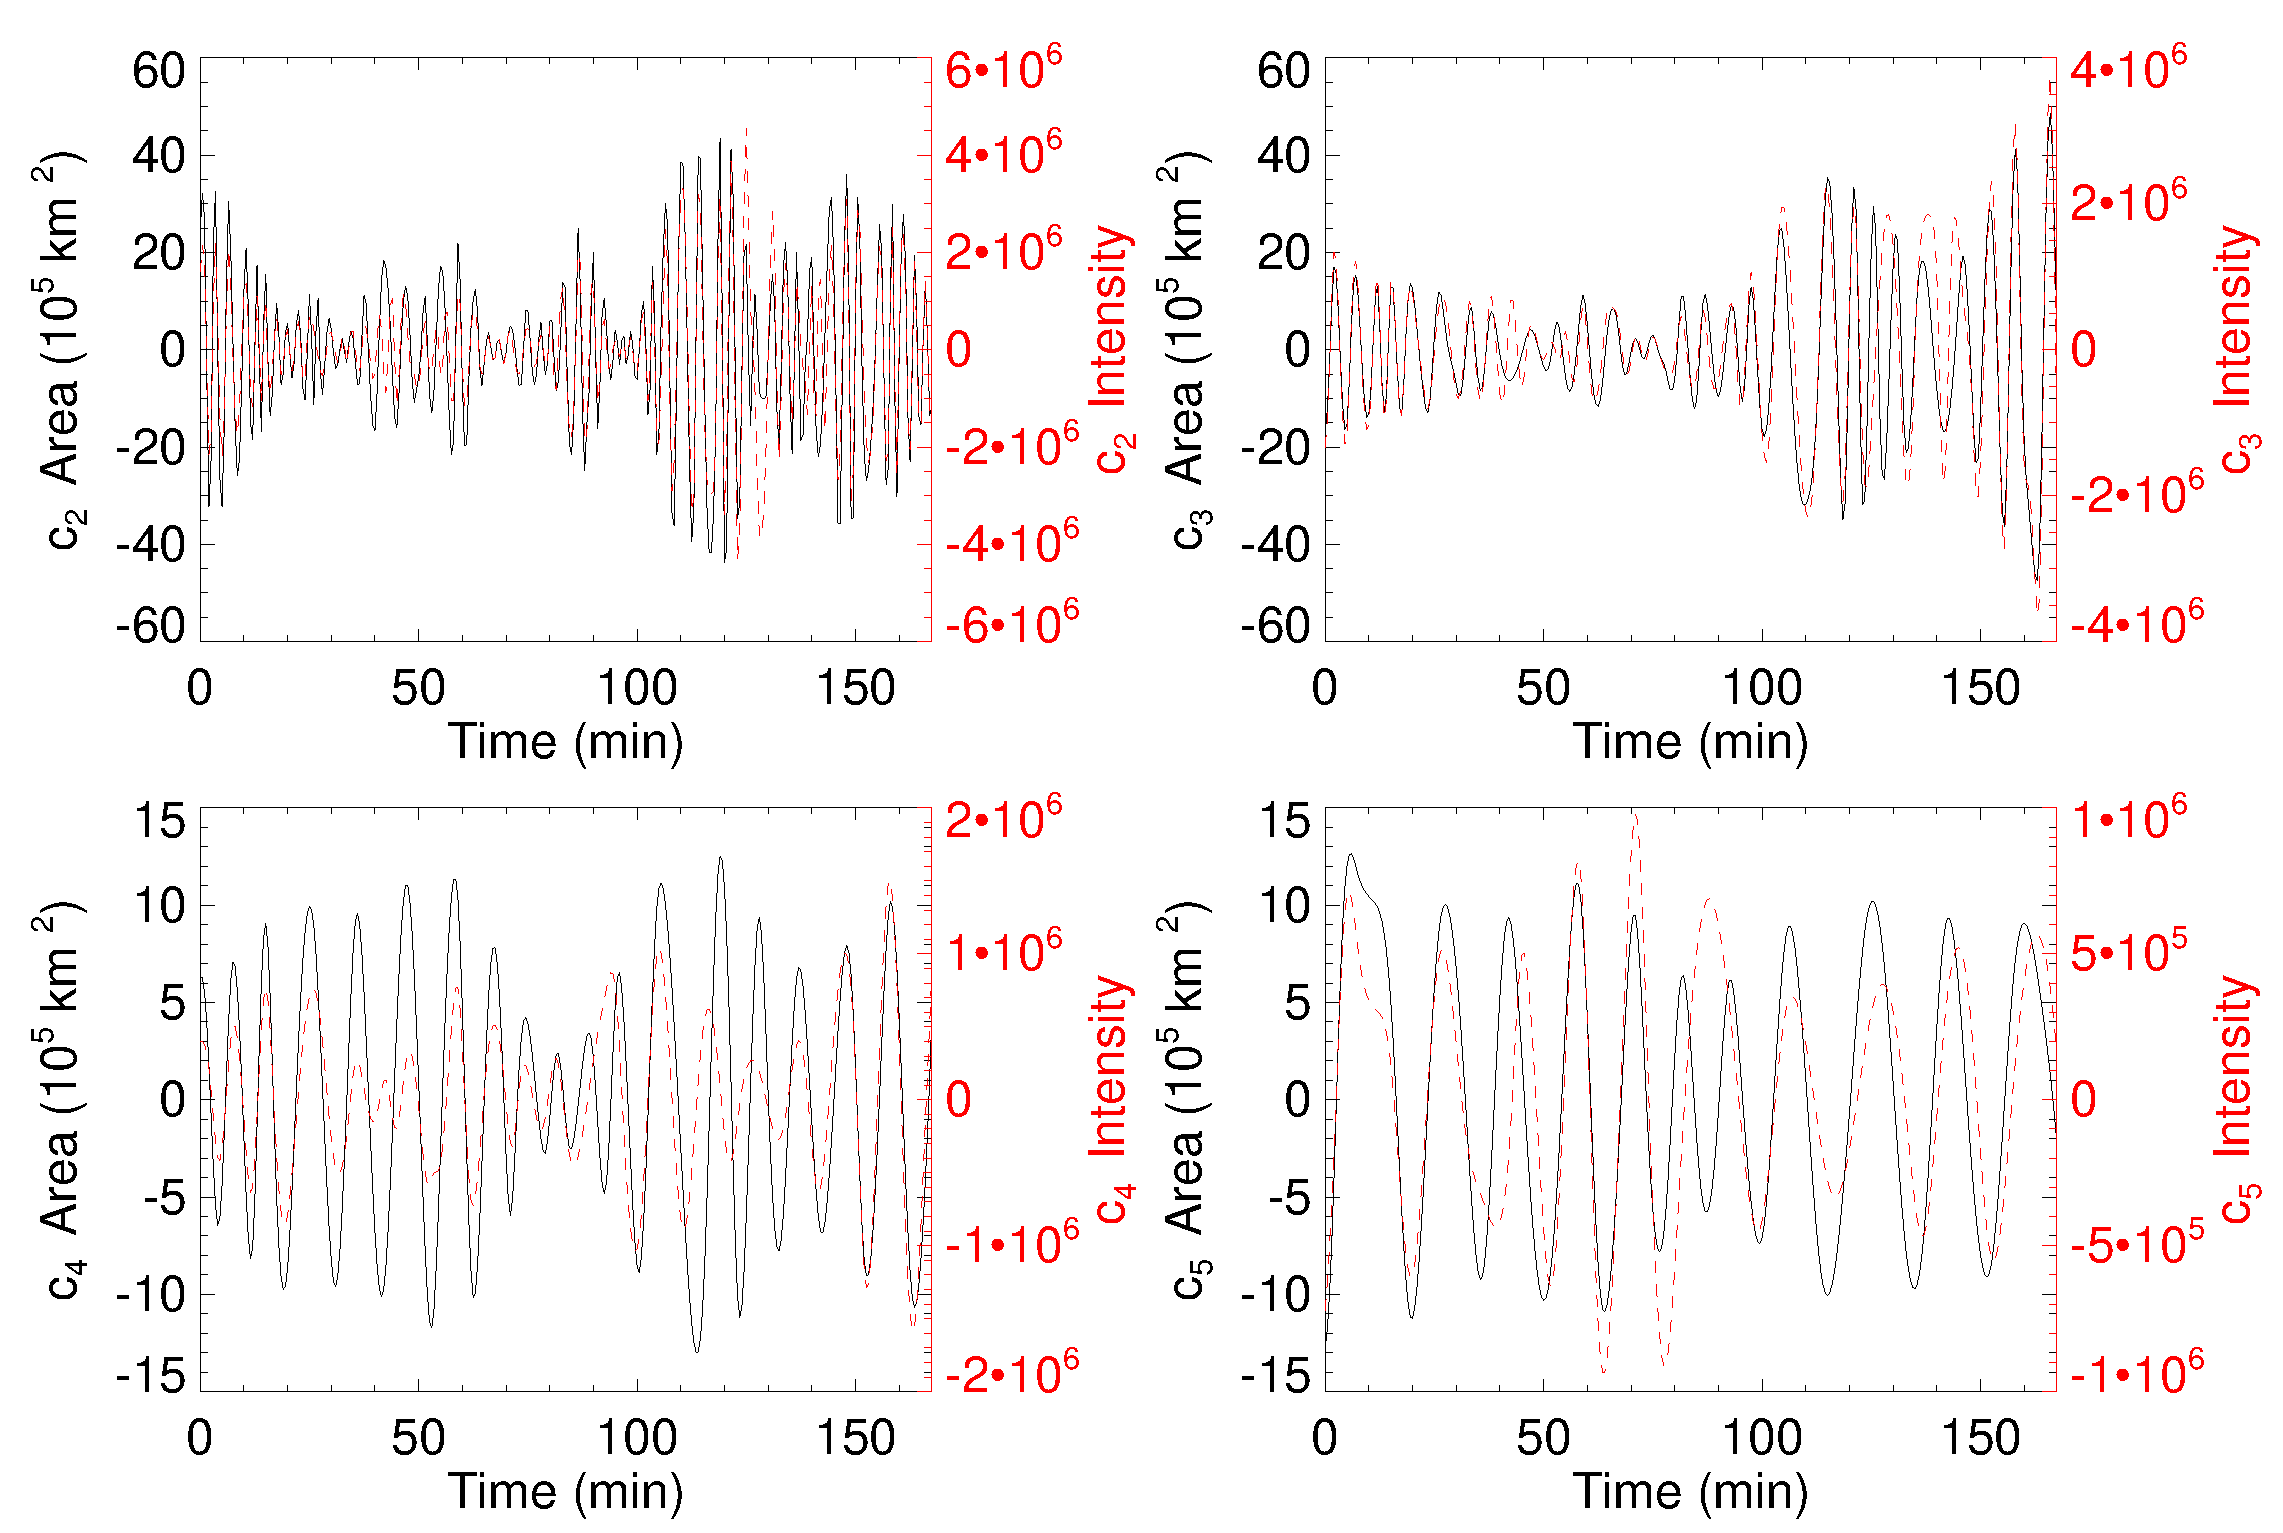
\includegraphics[width=\textwidth]{2005_IMFs.eps}
      \caption{
      			Same as Figure \ref{1999IMF} but for the sunspot in AR 10789 observed in 2005.
      		  }
      \label{20005IMF}
   \end{sidewaysfigure}
   
	Figure \ref{2005sunspot} shows the wavelet analysis of the 2005 sunspot area and intensity in AR 10789.
	There are four periods that exist at 95\% confidence level: 4, 7.5, 11, and 16.5 minutes.
	Each period has a region of high power in the wavelet, with the lower periods appearing nearer the end of the time series.
	The corresponding intensity wavelet reveals that there are three periods of 4, 7.5, and 10.5 minute oscillations; however, the 16.5-minute oscillation is present but is a very weak signal.
	The cross-wavelet phase indicates that these oscillations are in phase.
	There are no major regions of out of phase behaviour.
		
	Figure \ref{20005IMF} shows the IMFs for the area and the intensity of the sunspot data in AR 10789.
	In this case, each period is found by the EMD process. IMF $c_{2}$, IMF $c_{3}$, IMF $c_{4}$, and IMF $c_{5}$ correspond to the 4, 7.5, 11, and 16.5-minute oscillation periods, respectively.
	IMF $c_{2}$ displays extensive in phase behaviour throughout the time series, which is a strong indication of the slow sausage MHD wave at a period not too dissimilar to the global \textit{p}-mode oscillation.
	The region of interest is within the time interval of 90 to 130 minutes for IMF $c_{4}$, where the wavelet has these oscillations.
	The IMF shows clear in phase behaviour in this time interval.
	The overall phase relation between the area and intensity indicates the presence of slow sausage waves.
	
\subsection{Magnetic pore, 15 October 2008}

   \begin{sidewaysfigure}
   \centering
   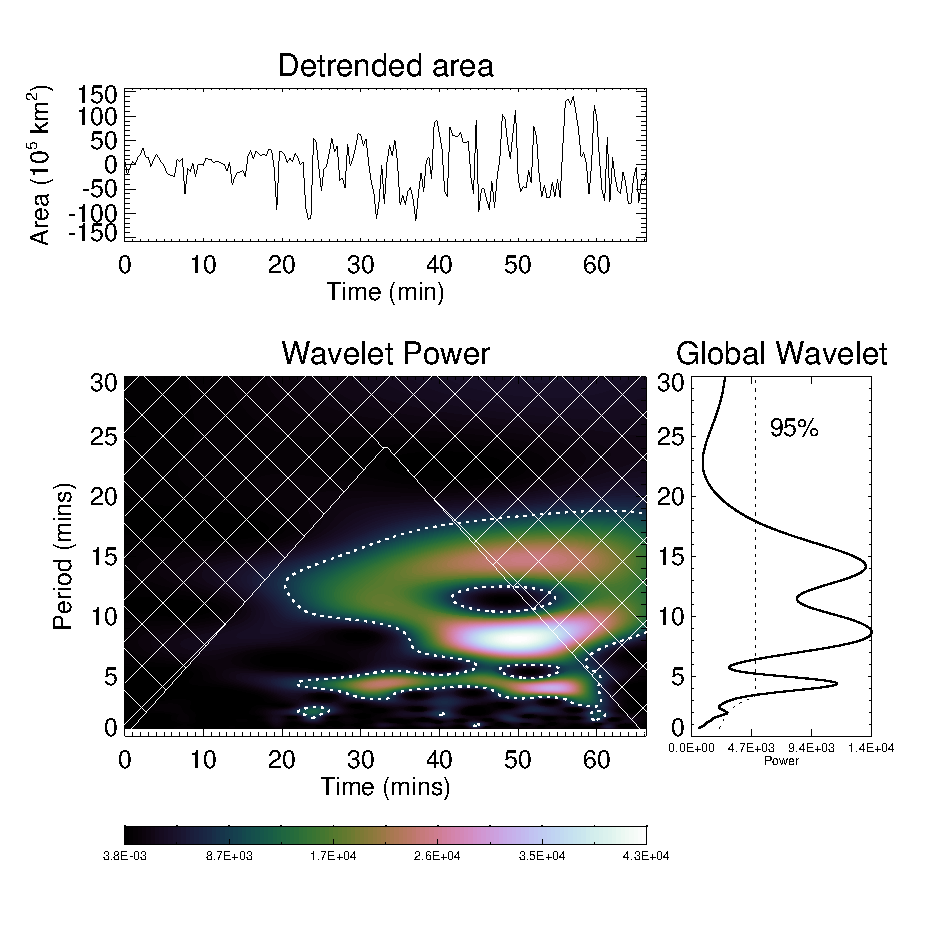
\includegraphics[width=0.49\textwidth]{2008_wl.eps}
   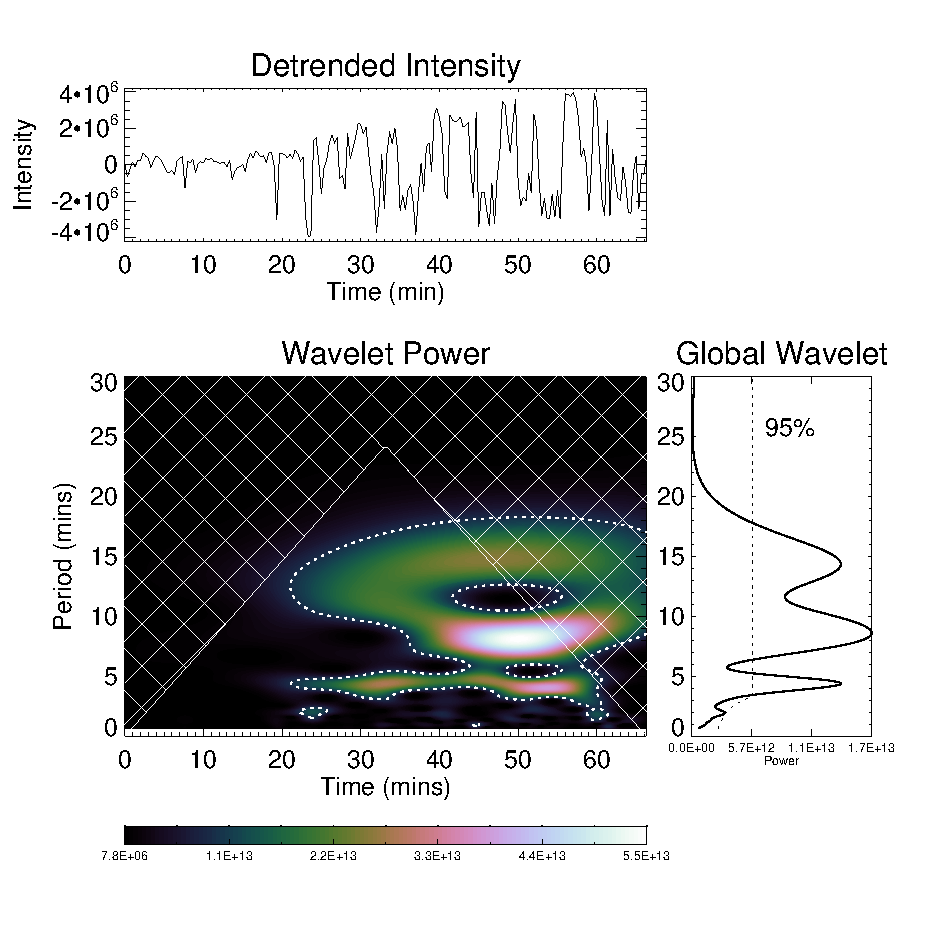
\includegraphics[width=0.49\textwidth]{2008_wl_inten.eps}
   	   \caption{
      			Same as Figure \ref{1999sunspot} but for the magnetic pore in AR 11005 observed in 2008.
 		      }
      \label{2008pore}
   \end{sidewaysfigure}
   
     \begin{sidewaysfigure}
     \centering
     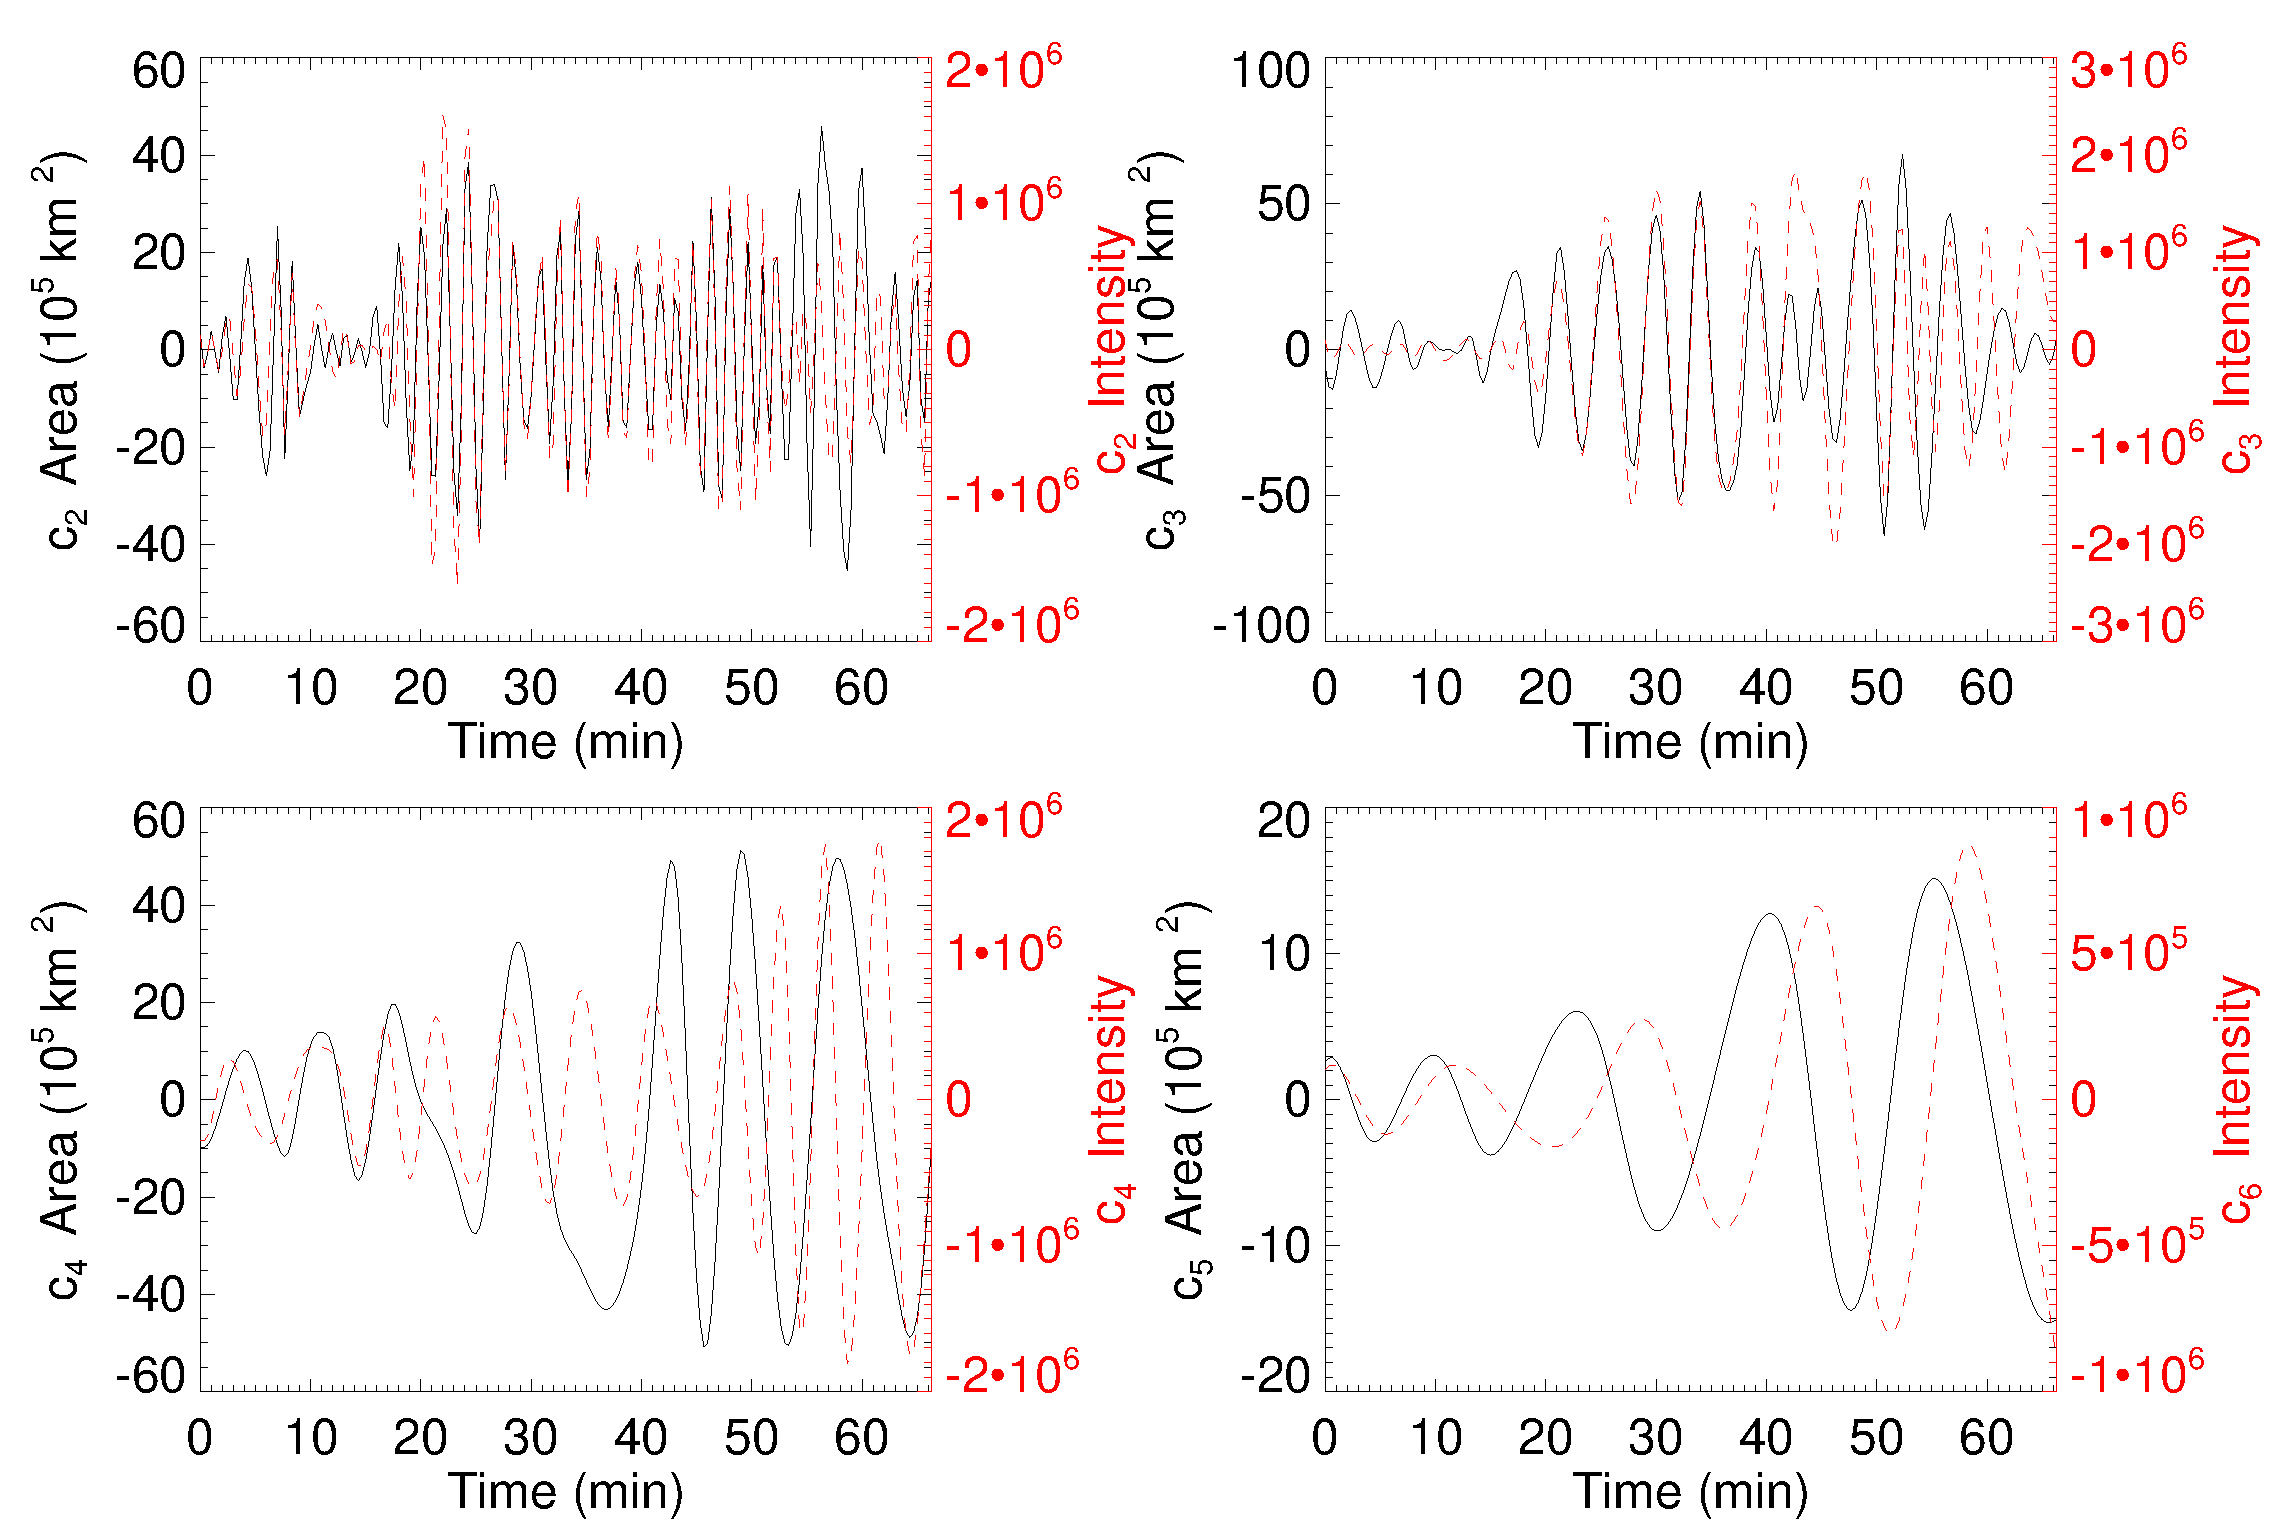
\includegraphics[width=\textwidth]{2008_IMFs.eps}
     \caption{
       			Same as Figure \ref{1999IMF} but for the magnetic pore in AR 11005 observed in 2008.
        		  }
     \label{20008IMF}
     \end{sidewaysfigure}
      
	Figure \ref{2008pore} shows the wavelet analysis of the magnetic pore with a light bridge.
	There are three periods that exist at 95 \% confidence level: 4.5, 8.5, and 14.5 minutes.
	The large part of the power of the period of 14-15 minutes is inside the COI; however, the period appears in the EMD analysis and has a large portion of power outside the COI and thus has not been ignored for this analysis.
	The three periods are seen in both area and intensity data when the wavelet analyses are cross-correlated.
	The power for these two periods is concentrated in the time interval of 20 to 60 minutes.
	The cross-wavelet analysis shows that the overlapping time span is somewhat smaller, at about 30 to 50 minutes.
	Furthermore, the wavelet power for each period runs parallel to each other throughout the time series, and they appear at the same time and seem to fade away at a similar time as well.
	
	Figure \ref{20008IMF} shows the IMFs for the area with intensity over-plotted.
	In this case, IMF $c_{3}$ indicates a period of 4.5 minutes and IMF $c_{4}$ has a characteristic period of 8.5 minutes, and this applies to both the area and intensity IMFs.
	IMF $c_{3}$ reveals that the phase relation is in phase for the majority of the time series.
	IMF $c_{4}$ reveals large regions of roughly in phase behaviour but with, again, a 45-degree phase difference.
	Not shown is the comparison of IMF $c_{4}$ and IMF $c_{5}$ for the area and intensity, respectively.
	At the end of the time series for both, there is a mixture of in phase behaviour but also with the intensity signal leading the area signal for the 8.5 minute oscillation.
	IMF $c_{5}$ and IMF $c_{6}$ for the area and intensity, respectively, show a period of 14.5 minutes.
	There is a region of near out of phase behaviour before this then turns into 45-degree phase difference with the area leading the intensity perturbations.
	Consistently, there are occurrences of unexplainable phase differences that require new MHD theory in order to explain.
       
	The easiest way to confirm the linearity of waves is to compare the amplitude of the oscillations to the characteristic scale of the structure.
	In all three cases studied here, the oscillation amplitudes are around 10\% or less of the total area, which indicates that these oscillations are linear.
	Furthermore, the amplitude of the oscillation in the last two cases is by and large the same, so the amplitude has scaled with the size of the structure.
	However, for the 1999 sunspot, the amplitude of the oscillation is an order of a magnitude less. Whether this is due to the large size of the sunspot or the very stable nature during the observation window needs to be investigated in future work.
	
\subsection{Standing harmonics}

	\begin{table}
	\centering
	\begin{tabular}{ccccc}
		\hline
		Dataset & & Period (Mins) & Ratio ($P_{1}/P_{i}$) & Expected Ratio \\ \hline \hline
		\multirow{4}{*}{Sunspot 1999} & $P_{1}$ & 32 $\pm$ 2.5 & - & -\\
							  		  & $P_{2}$ & 16 $\pm$ 1.5 & 2 $\pm$ 0.2 & 2\\
							  		  & $P_{3}$ & 7 $\pm$ 0.5 & 4.6 $\pm$ 0.3 & 3\\
							  		  & $P_{4}$ & 4 $\pm$ 0.5 & 8 $\pm$ 0.5 & 4\\ \hline
		\multirow{4}{*}{Sunspot 2005} & $P_{1}$ & 16.5 $\pm$ 1.5  & - & -\\
					      			  & $P_{2}$ & 11 $\pm$ 0.5 & 1.5 $\pm$ 0.2 & 2\\
					      			  & $P_{3}$ & 7.5 $\pm$ 0.5 & 2.2 $\pm$ 0.2 & 3\\
					      			  & $P_{4}$ & 4 $\pm$ 0.5 & 4.2 $\pm$ 0.6 & 4\\ \hline
		\multirow{4}{*}{Pore 2008}    & $P_{1}$ & 14.5 $\pm$ 0.5 & - & -\\
		 							  & $P_{2}$ & 8.5 $\pm$ 0.5 & 1.7 $\pm$ 0.1 & 2\\
					      			  & $P_{3}$ & 4.5 $\pm$ 0.5 & 3.2 $\pm$ 0.2 & 3\\ \hline
	\end{tabular}
		\caption{The periods of oscillations that are found in the area of the waveguides that exist at 95\% confidence level.}
		\label{chap3:harm_table}
	\end{table}
		
	Basic MHD theory interpretation allows sunspots and magnetic pores to be described as vertical cylindrical flux tubes, with the base bounded in the photosphere and the top bounded at the transition region due to the sharp gradients in the plasma properties at these locations.
	Taking this further, an ideal flux tube is assumed here.
	The plasma density and magnetic field are homogeneous within the flux tube.
	This means that the standing harmonics of such flux tubes are the MHD equivalent to the harmonics in an closed-ended compressible air pipe, where the ratio of the harmonic periods is given by \, $P_{1}/P_{2}=2, \,\, P_{1}/P_{3}=3$, and so forth.
	This only applies in the long-wavelength or thin-tube approximation.
	Using harmonic ratios to carry out magneto-seismology has been used, for example, by \citet{2005ApJ...624L..57A,2005A&A...430.1109A} who researched the effects of longitudinal density stratification on kink oscillations and resonantly damped kink oscillations, while \citet{luna-cardozo} studied longitudinal density effects and loop expansion on the slow sausage MHD wave.
	\citet{luna-cardozo} found that specific density profiles in lower atmospheric flux tubes could increase or decrease the value of the period ratio.
	The authors are unaware of any work that gives the changes to further harmonic ratios, so the assumption that the amount of deviation from the canonical value for the period ratio ($P_{1}/P_{2}$) is the same for other period ratios; e.g., $P_{1}/P_{3}$ or higher is used.
	
	We now summarise the observed findings. Table \ref{chap3:harm_table} contains the periods of oscillations found in all three magnetic waveguides.
	There are four periods found for the 1999 sunspot.
	The second period of 16 minutes gives a period ratio ($P_{1}/P_{2}$) of 2 $\pm$ 0.2, which is exactly the same as the expected value of a uniform waveguide with a canonical value of 2.
	The next period ratio is 4.6 $\pm$ 0.3.
	Here, the change from canonical value is substantial if this is indeed the third period, which should be around 10.6 minutes, unless the effect on the harmonic ratio increases with each successive ratio.
	The last period is difficult to incorporate into the harmonic standpoint, and it is most likely that the four-minute period is due the global \textit{p}-mode.
	
	For the 2005 sunspot in AR 10789, there is a clearer picture of potential harmonics.
	The first period is 16.5 minutes and the second period is 11 minutes, which gives a ratio of 1.5 $\pm$ 0.2, and the third period of 7.5 minutes gives a ratio of 2.2 $\pm$ 0.3.
	The period ratio is modified downwards in a consistent manner as the harmonic number increases.
	These ratios are strong evidence of standing waves in this magnetic waveguide.
	As was the case for the 1999 sunspot, the period at four minutes has a period ratio that does not fit into this harmonic viewpoint and is most likely due to the global \textit{p}-mode instead.
	
	For the 2008 pore of AR 11005, the picture is more muddled by the shorter time series.
	Taking the 15-minute period to be the first harmonic, the ratio is 1.7 $\pm$ 0.1 for the 8.5-minute period, very similar to both first-period ratios of the previous sunspots.
	The third period is again very close to the period of the global \textit{p}-mode and does not fit into the harmonic viewpoint.
	
	The main conclusion to take away from this data analysis at this point is that the simple homogeneous flux tube model cannot fully account for these ratios.
	However, this simple model seems to be robust enough to give a good first insight.
	The most likely reasons for deviation from the canonical period ratio value are, firstly, that sunspots and magnetic pores (just like most lower atmospheric magnetic structures) expand with height, causing magnetic stratification \citep{2008A&A...486.1015V,luna-cardozo}, and secondly, that the Sun's gravity causes density stratification \citep{Andries2009}.
	These two effects will either increase or decrease the period ratio of the harmonics depending on the chosen density or magnetic profile (see \citet{luna-cardozo} for a detailed analysis in the context of slow sausage oscillations or see \citet{2013SoPh..tmp..195E} for kink modes).
	In addition, these magnetic structures are rarely purely cylindrical, but can be elliptical (or arbitrary) in shape \citep[see][]{Ruderman2009,2009A&A...502..315M} and in most cases are non-axially symmetric.
	Also, in some cases the flux tube is more suitably described as closed-ended at the photosphere and open-ended at the transition region, which would remove the even harmonics.
	 
\section{Conclusions}

	In this chapter we have investigated three magnetic waveguides with the objective of detecting MHD sausage waves and determining whether they are slow or fast, propagating or standing.
	Based on the results presented here, we confidently interpreted the observed periodic changes in the cross-sectional area of these flux tubes, which are manifested as a magnetic pore and two sunspot waveguide structures, as proof of the existence of linear slow and fast surface sausage MHD oscillations.
	Using wavelet analysis, we found standing waves in the photosphere with periods ranging from 4 to 32 minutes.
	Employing complementary EMD analysis has allowed the detected MHD modes to be identified as a combination of \textit{fast surface sausage} and \textit{slow sausage} modes, thanks to the phase difference of the area and intensity.
	It is very likely that these oscillations are \textit{standing harmonics} supported in a flux tube.
	The period ratio ($P_{1}/P_{i=2,3}$) of these oscillations indicates strongly that they are part of a group of standing harmonics in a flux tube that is non-homogeneous and bound by the photosphere and the transition region.
	Furthermore, there is possible indirect evidence of mode conversion occurring in one of these magnetic waveguides.